\section{Tournament Analysis}\label{tournament-analysis}

\begin{frame}{Mean Scores and Coefficient of Variation}

\begin{figure}[htbp]
\centering
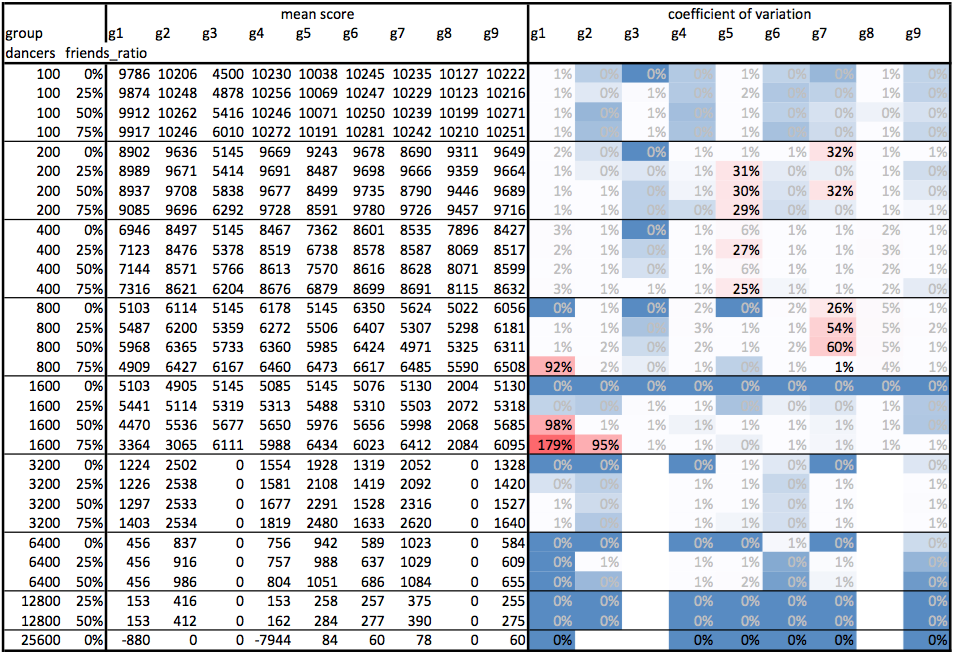
\includegraphics{imgs/mean-cov.png}
\caption{Mean Scores and Coefficient of Variation\label{img-mean-cov}}
\end{figure}

\end{frame}

\begin{frame}{Big Variations for g2}

\begin{itemize}
\tightlist
\item
  variation is generally pretty low ( \textless{} 1\% )
\item
  For g2, huge variation of 95\% for (1600, 75\%)
\end{itemize}

\begin{longtable}[c]{@{}lrrcr@{}}
\toprule
& dancers & friends & group & score\tabularnewline
\midrule
\endhead
1791 & 1600 & 1200 & g2 & 6024\tabularnewline
1792 & 1600 & 1200 & g2 & 141\tabularnewline
1793 & 1600 & 1200 & g2 & 5925\tabularnewline
1794 & 1600 & 1200 & g2 & 141\tabularnewline
1795 & 1600 & 1200 & g2 & 141\tabularnewline
1796 & 1600 & 1200 & g2 & 5967\tabularnewline
1797 & 1600 & 1200 & g2 & 141\tabularnewline
1798 & 1600 & 1200 & g2 & 141\tabularnewline
1799 & 1600 & 1200 & g2 & 6017\tabularnewline
1800 & 1600 & 1200 & g2 & 6016\tabularnewline
\bottomrule
\end{longtable}

\end{frame}

\begin{frame}{Big Variations for g2}

\begin{itemize}
\tightlist
\item
  because of estimating friend density for our Medium Strategy
\item
  dance with partners for longer duration
\item
  competitive score of 5989.80 in half the scenarios
\item
  meagre 141 for the rest
\item
  50\% chance that the unluckiest dancer will not find friends
\item
  Because of the uncertainty, better off just ignoring friends
\item
  should try to ensure that every dancer dances
\end{itemize}

\end{frame}

\begin{frame}{Big Variations for g1 and g7}

\begin{itemize}
\tightlist
\item
  also see a huge variation because of claustrophobia.
\item
  Other high variations are due to single outliers (on the worse side)
  in data.
\end{itemize}

\begin{longtable}[c]{@{}lrrcr@{}}
\toprule
& dancers & friends & group & score\tabularnewline
\midrule
\endhead
1360 & 800 & 200 & g7 & -3230\tabularnewline
1437 & 800 & 400 & g7 & -2776\tabularnewline
1468 & 800 & 600 & g1 & -8686\tabularnewline
1702 & 1600 & 800 & g1 & -8688\tabularnewline
1781 & 1600 & 1200 & g1 & -8687\tabularnewline
1782 & 1600 & 1200 & g1 & -8686\tabularnewline
2388 & 25600 & 0 & g1 & -880\tabularnewline
2391 & 25600 & 0 & g4 & -7944\tabularnewline
\bottomrule
\end{longtable}

\end{frame}

\begin{frame}{Tournament categories}

\begin{itemize}
\tightlist
\item
  Small

  \begin{itemize}
  \tightlist
  \item
    for \(d<=800\)
  \item
    It is possible to systematically find soulmates
  \end{itemize}
\item
  Medium

  \begin{itemize}
  \tightlist
  \item
    for \(800 < d <=1600\)
  \item
    It is possible for all dancers to dance at the same time on the
    dance floor
  \end{itemize}
\item
  Large

  \begin{itemize}
  \tightlist
  \item
    for \(1600 < d\)
  \item
    We require some sort of scheduling to ensure each of the dancer gets
    to dance
  \item
    none of the dancers should suffer claustrophobia
  \end{itemize}
\end{itemize}

\end{frame}

\begin{frame}{Team wise Scores}

\begin{figure}[htbp]
\centering
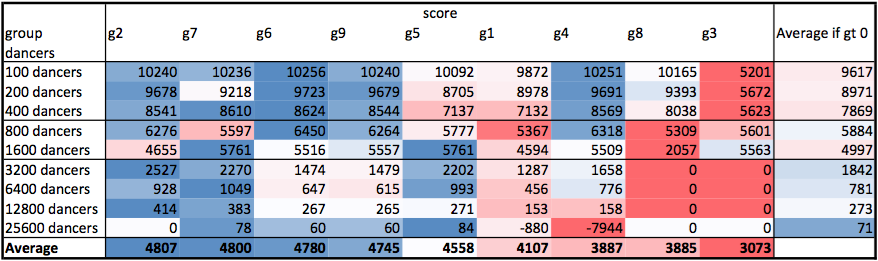
\includegraphics{imgs/team-scores.png}
\caption{Scores of teams per number of dancers\label{team-scores}}
\end{figure}

\begin{itemize}
\tightlist
\item
  each row is a heat map, blue being better score
\item
  \textbf{Our group (g2) scores the best Average}, closely followed by
  g7
\item
  Next best score is by g6 and g9, which share a rather noticable
  correlation!
\end{itemize}

\end{frame}

\begin{frame}{Team categories}

\begin{itemize}
\tightlist
\item
  g1 and g7

  \begin{itemize}
  \tightlist
  \item
    score well on all categories
  \item
    thus score highest and second higher respectively
  \end{itemize}
\item
  g6, g9, g4

  \begin{itemize}
  \tightlist
  \item
    score well on small category
  \end{itemize}
\item
  g5

  \begin{itemize}
  \tightlist
  \item
    scores well on Large category
  \item
    but fails to perform on Small
  \end{itemize}
\end{itemize}

\end{frame}

\begin{frame}{Relative Performance}

\begin{figure}[htbp]
\centering
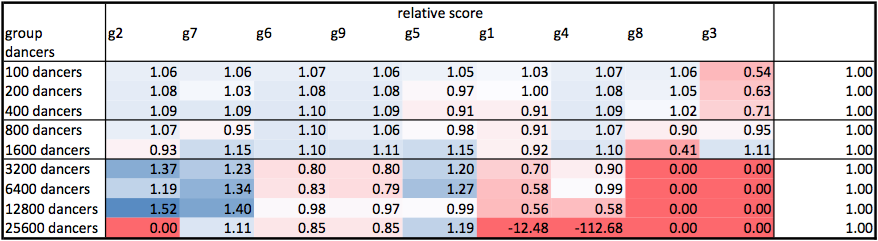
\includegraphics{imgs/team-rel.png}
\caption{Relative scores of teams per number of dancers\label{team-rel}}
\end{figure}

\end{frame}

\begin{frame}{Relative Performance}

\begin{figure}[htbp]
\centering
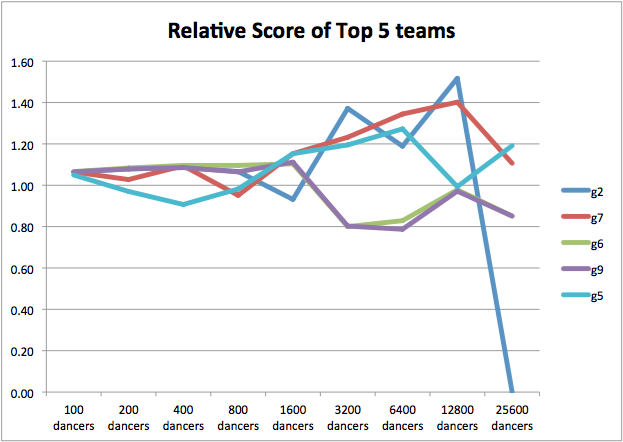
\includegraphics{imgs/team-5-rel.png}
\caption{Plot of relative scores of top 5 teams\label{team-5-rel}}
\end{figure}

\end{frame}

\begin{frame}{Relative Performance}

\begin{itemize}
\tightlist
\item
  strength is relatively stronger scores in Large category
\item
  to order, we follow a simple average, which seems to favor Small
  category
\item
  Yet we achieve the highest overall average
\item
  testimony to our performance across categories
\end{itemize}

\end{frame}

\begin{frame}{Performance in Large category}

\begin{itemize}
\tightlist
\item
  For Large category, our strategy has step behavior
\item
  g7 seems to have a more continuous looking behavior 
\end{itemize}

\begin{longtable}[c]{@{}rrrrr@{}}
\toprule
\begin{minipage}[b]{0.12\columnwidth}\raggedleft\strut
friends
\strut\end{minipage} &
\begin{minipage}[b]{0.16\columnwidth}\raggedleft\strut
batch size
\strut\end{minipage} &
\begin{minipage}[b]{0.17\columnwidth}\raggedleft\strut
num batches
\strut\end{minipage} &
\begin{minipage}[b]{0.18\columnwidth}\raggedleft\strut
target score
\strut\end{minipage} &
\begin{minipage}[b]{0.23\columnwidth}\raggedleft\strut
num dancing cols
\strut\end{minipage}\tabularnewline
\midrule
\endhead
\begin{minipage}[t]{0.12\columnwidth}\raggedleft\strut
3200
\strut\end{minipage} &
\begin{minipage}[t]{0.16\columnwidth}\raggedleft\strut
1680
\strut\end{minipage} &
\begin{minipage}[t]{0.17\columnwidth}\raggedleft\strut
2
\strut\end{minipage} &
\begin{minipage}[t]{0.18\columnwidth}\raggedleft\strut
2545
\strut\end{minipage} &
\begin{minipage}[t]{0.23\columnwidth}\raggedleft\strut
42
\strut\end{minipage}\tabularnewline
\begin{minipage}[t]{0.12\columnwidth}\raggedleft\strut
6400
\strut\end{minipage} &
\begin{minipage}[t]{0.16\columnwidth}\raggedleft\strut
1520
\strut\end{minipage} &
\begin{minipage}[t]{0.17\columnwidth}\raggedleft\strut
5
\strut\end{minipage} &
\begin{minipage}[t]{0.18\columnwidth}\raggedleft\strut
1002
\strut\end{minipage} &
\begin{minipage}[t]{0.23\columnwidth}\raggedleft\strut
38
\strut\end{minipage}\tabularnewline
\begin{minipage}[t]{0.12\columnwidth}\raggedleft\strut
12800
\strut\end{minipage} &
\begin{minipage}[t]{0.16\columnwidth}\raggedleft\strut
1280
\strut\end{minipage} &
\begin{minipage}[t]{0.17\columnwidth}\raggedleft\strut
10
\strut\end{minipage} &
\begin{minipage}[t]{0.18\columnwidth}\raggedleft\strut
439
\strut\end{minipage} &
\begin{minipage}[t]{0.23\columnwidth}\raggedleft\strut
32
\strut\end{minipage}\tabularnewline
\begin{minipage}[t]{0.12\columnwidth}\raggedleft\strut
25600
\strut\end{minipage} &
\begin{minipage}[t]{0.16\columnwidth}\raggedleft\strut
720
\strut\end{minipage} &
\begin{minipage}[t]{0.17\columnwidth}\raggedleft\strut
36
\strut\end{minipage} &
\begin{minipage}[t]{0.18\columnwidth}\raggedleft\strut
105
\strut\end{minipage} &
\begin{minipage}[t]{0.23\columnwidth}\raggedleft\strut
18
\strut\end{minipage}\tabularnewline
\bottomrule
\end{longtable}

\begin{itemize}
\tightlist
\item
  claustrophobia to mitigate: -50 = 16 turns
\item
  target score: 105 = 35 turns
\item
  50 turns for dancing per batch
\item
  10 turns for moving per batch
\item
  1800 / 60 = 30 batches can be handled
\end{itemize}

\end{frame}
